% !TEX root =  master.tex
\chapter{Evaluation}\label{chapter:evaluation}


\section{Evaluation of ResNeXt} \label{chapter:eval_resnext}
\sectionauthor{Written by Tobias Richstein}

The training of the ResNeXt went very well. As can be seen in figure \vref{fig:resnext_eval} the relevant metrics of Accuracy, F1 score, Recall and precision keep going up during training. Now it is important to stress two things: First, we are not actually too interested in getting perfect results from this model in terms of classifying the 14 illnesses from the NIH dataset (from section \vref{data:nih}) and second, the number of samples is heavily unbalanced and most images have no findings at all. Especially the second fact explains the rather low recall score (ratio of true positive predictions in a class to all observations of that class) and the resulting low F1 score.

\begin{figure*}[h]
	\centering
	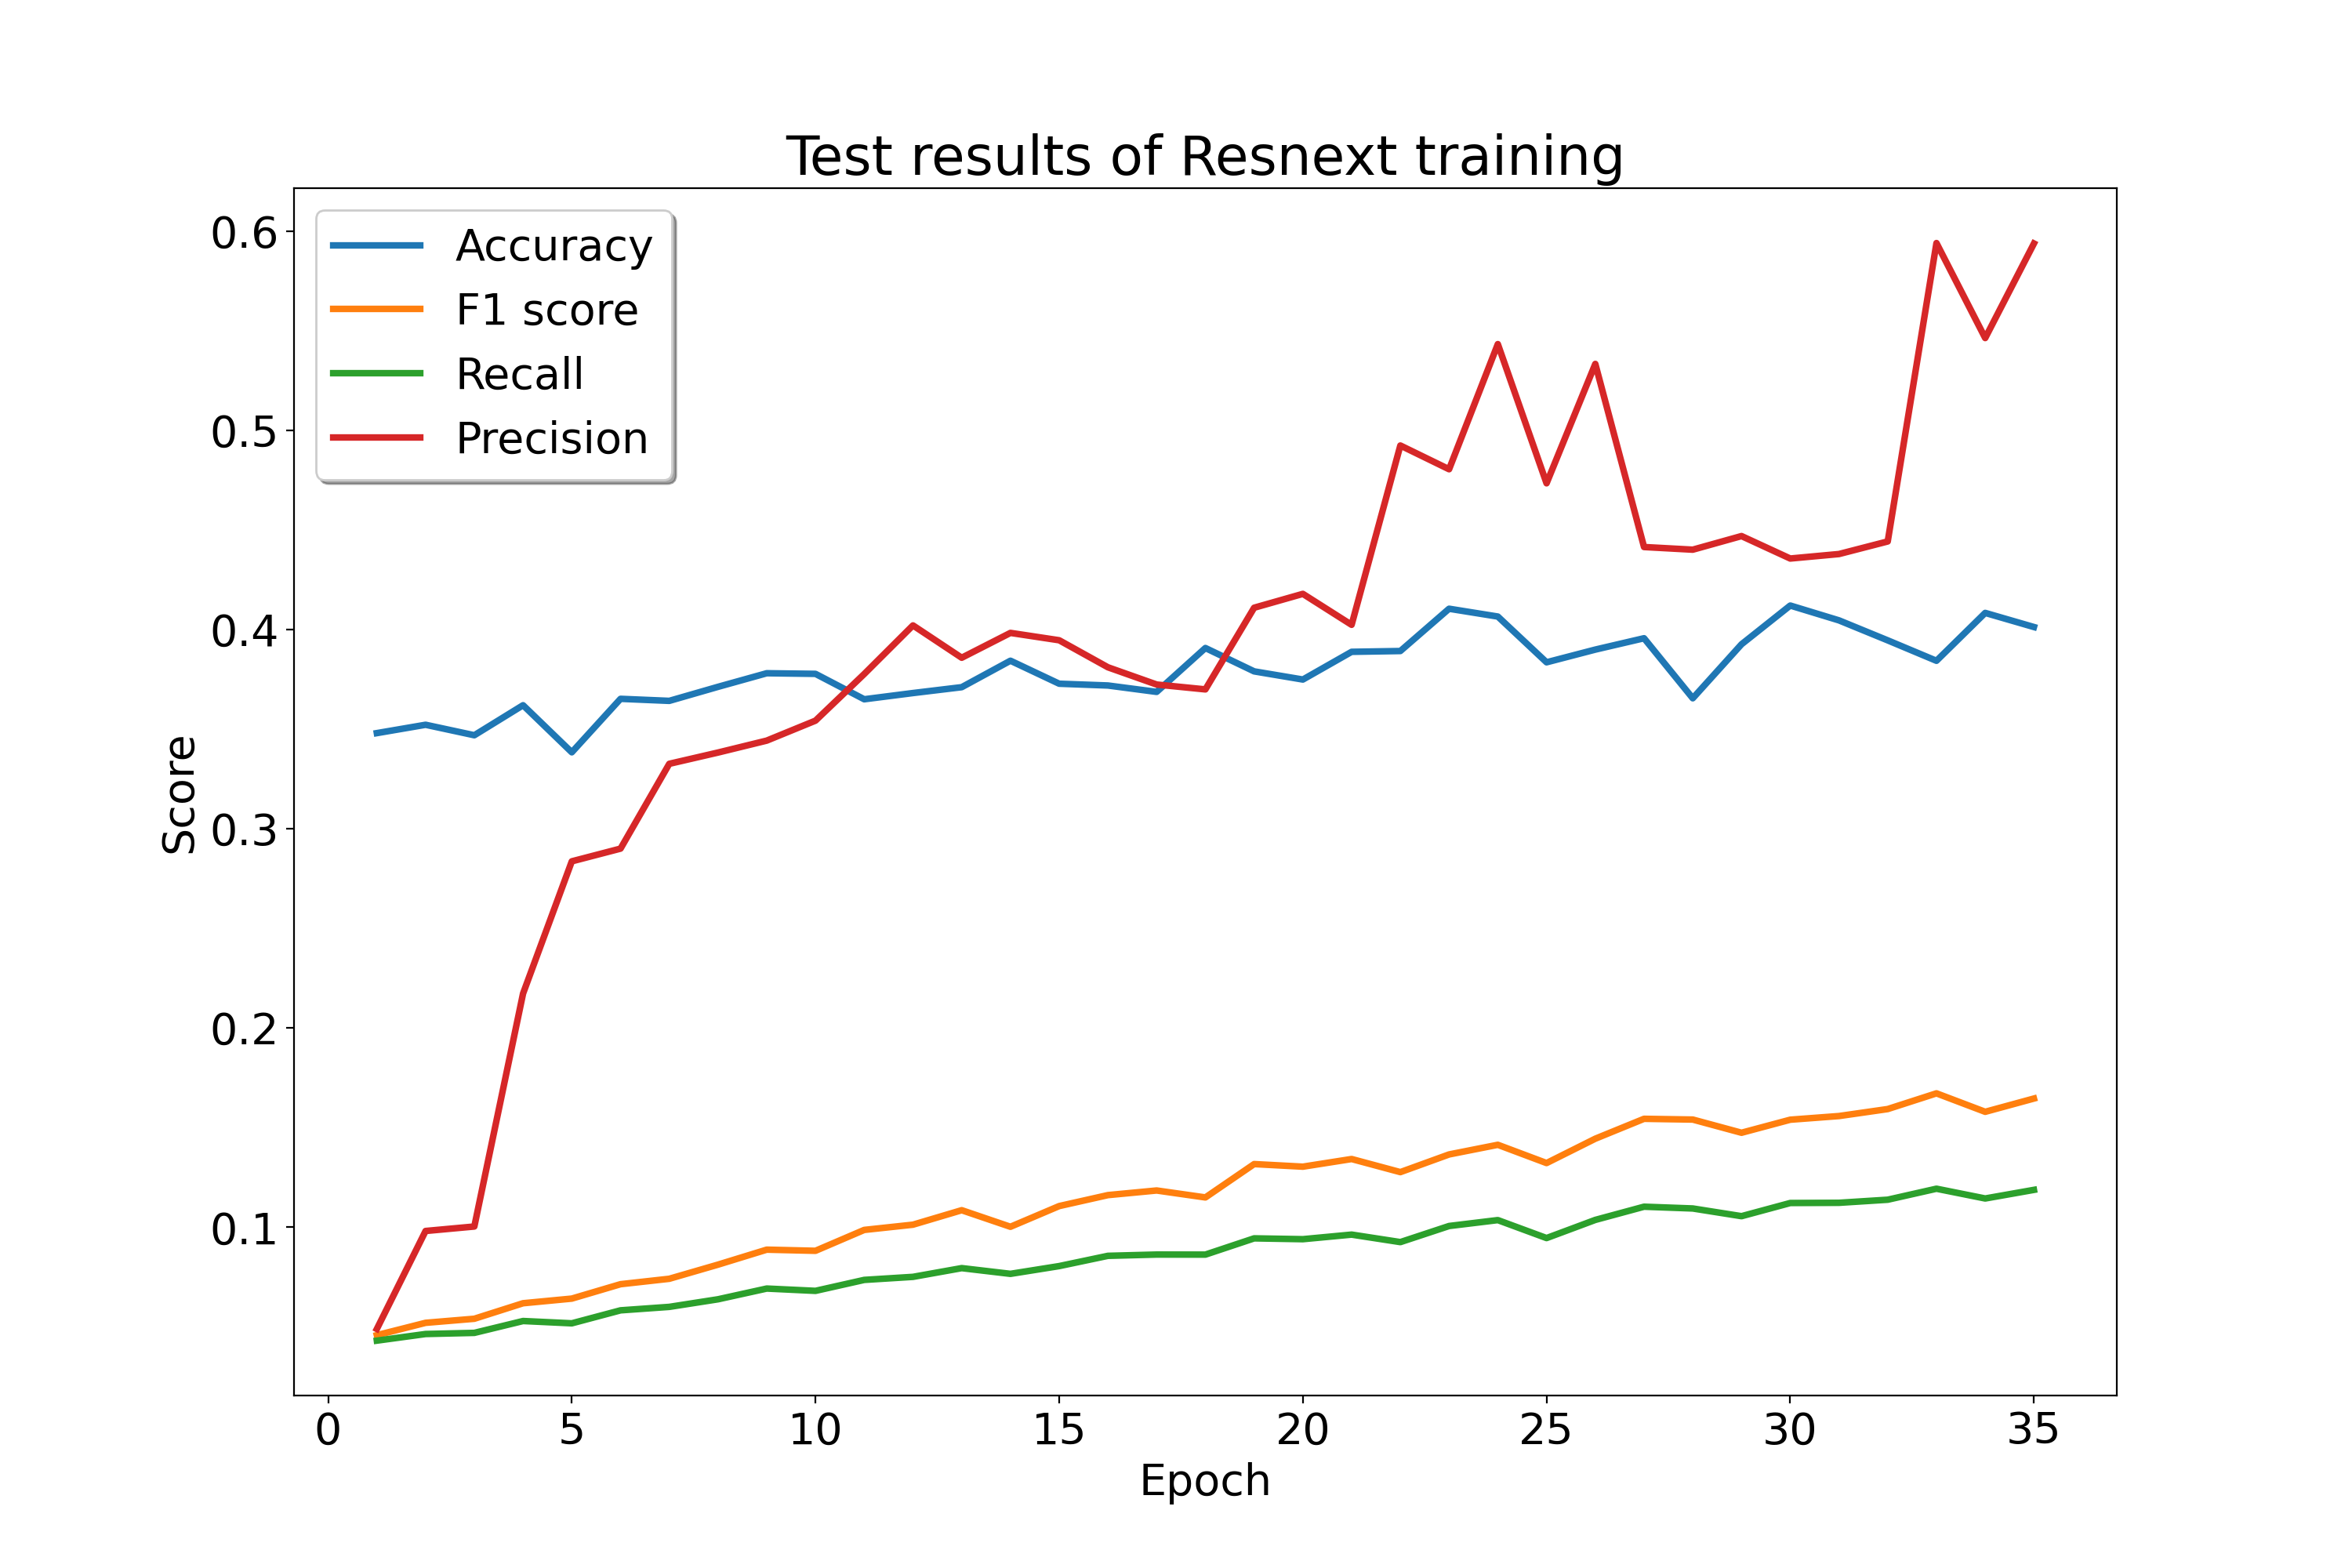
\includegraphics[width=.8\linewidth]{img/test_results_backbone_rcnn_35.png}
	\caption{ResNeXt model metrics during training}
	\label{fig:resnext_eval}
\end{figure*}

In a more refined setup we could have modified the dataloader to for example over-sample all underrepresented or on the other hand under-sample some of the dominant illness labels found in the dataset to balance the training a little more. Since again we are not really interested in the actual classification but more in the feature vectors that we can use as the Faster R-CNN backbone, we are satisfied with a final Precision of $0.59$, Recall of $0.12$, Accuracy of $0.40$ and F1 score of $0.16$. We could also certainly have trained the model further as no dramatic overfit seems to have occurred yet but as will be shown in the next section, the overall results for which we need the backbone are quite satisfactory.

\section{Evaluation of COVID-19 detection}\label{chapter:eval_rcnn_yolo}
\sectionauthor{Written by Julian Seibel}
For evaluating our COVID-19 detection capabilities, we identified two major steps that include the evaluation of the prediction quality for both the detection models, namely Faster \ac{R-CNN} and \ac{YOLO} and the evaluation of our ensemble approach, where we applied the method described previously in \ref{section:combining_detections} to come up with a final prediction considering both model outputs. 

There are multiple metrics possible for measuring the quality of an object detection model. However, we decided to use the widely used \acl{mAP} (mAP) as our crucial performance evaluation metric since many of the contributions in the field of object detection adapted the metric becoming the de-facto standard in many open opject detection challenges like Pascal VOC \autocite{everingham2010pascal} or COCO \autocite{coco}. The \ac{mAP} considers both, the quality of the class prediction as well as the quality of the bounding box prediction. Regarding the latter, the \ac{IoU} between ground truth and prediction is used to measure the placement quality by defining a threshold $t$ which determines if a predicted box will be handled as true positive (\ac{IoU} $> t$) or as false positive (\ac{IoU} $< t$)\footnote{Since it is not necessary to count true negatives as there should just be no box, those values will be excluded also in the computation of recall and precision later on.}. There are various values for $t$ conceivable depending also on the requirements the model needs to fulfill. In general the threshold used is denoted as \ac{mAP}@$t$. In our example we mainly focused on the \ac{mAP}@$.50$ score. Hence, a predicted bounding box will be count as true positive if the \ac{IoU} value indicates a 50\% coverage of the ground truth. There are different ways to calculate the final \ac{mAP} score, for example in \autocite{padilla2020survey} the authors proposed to use a all-point interpolation method to smooth the precision-recall curve to calculate the final average precision. Since our work only considers one class bounding box prediction (\enquote{opacity}), the \ac{mAP} is reduced to just the average precision (AP).

First, we consider both the models and compare them in terms of our selected metrics in our validation phase that is performed after each training epoch.
For the \ac{YOLO} model, figure \ref{fig:yolo_pretraining_results} shows the validation metrics during pretraining on the \ac{RSNA} data. The graph shows that during the first epochs of the pretraining the metric values increase but then kind of flatten out achieving almost $\approx60\%$ in \ac{mAP}@$.50$. Similar to the ResNeXt backbone model, we are not particularly interested in achieving state-of-the-art scores during pretraining, rather that we experience a continuous learning for \enquote{introducing} the model and its weights to the problem domain.
\begin{figure*}[h!]
	\begin{minipage}[b]{.5\linewidth} % [b] => Ausrichtung an \caption
		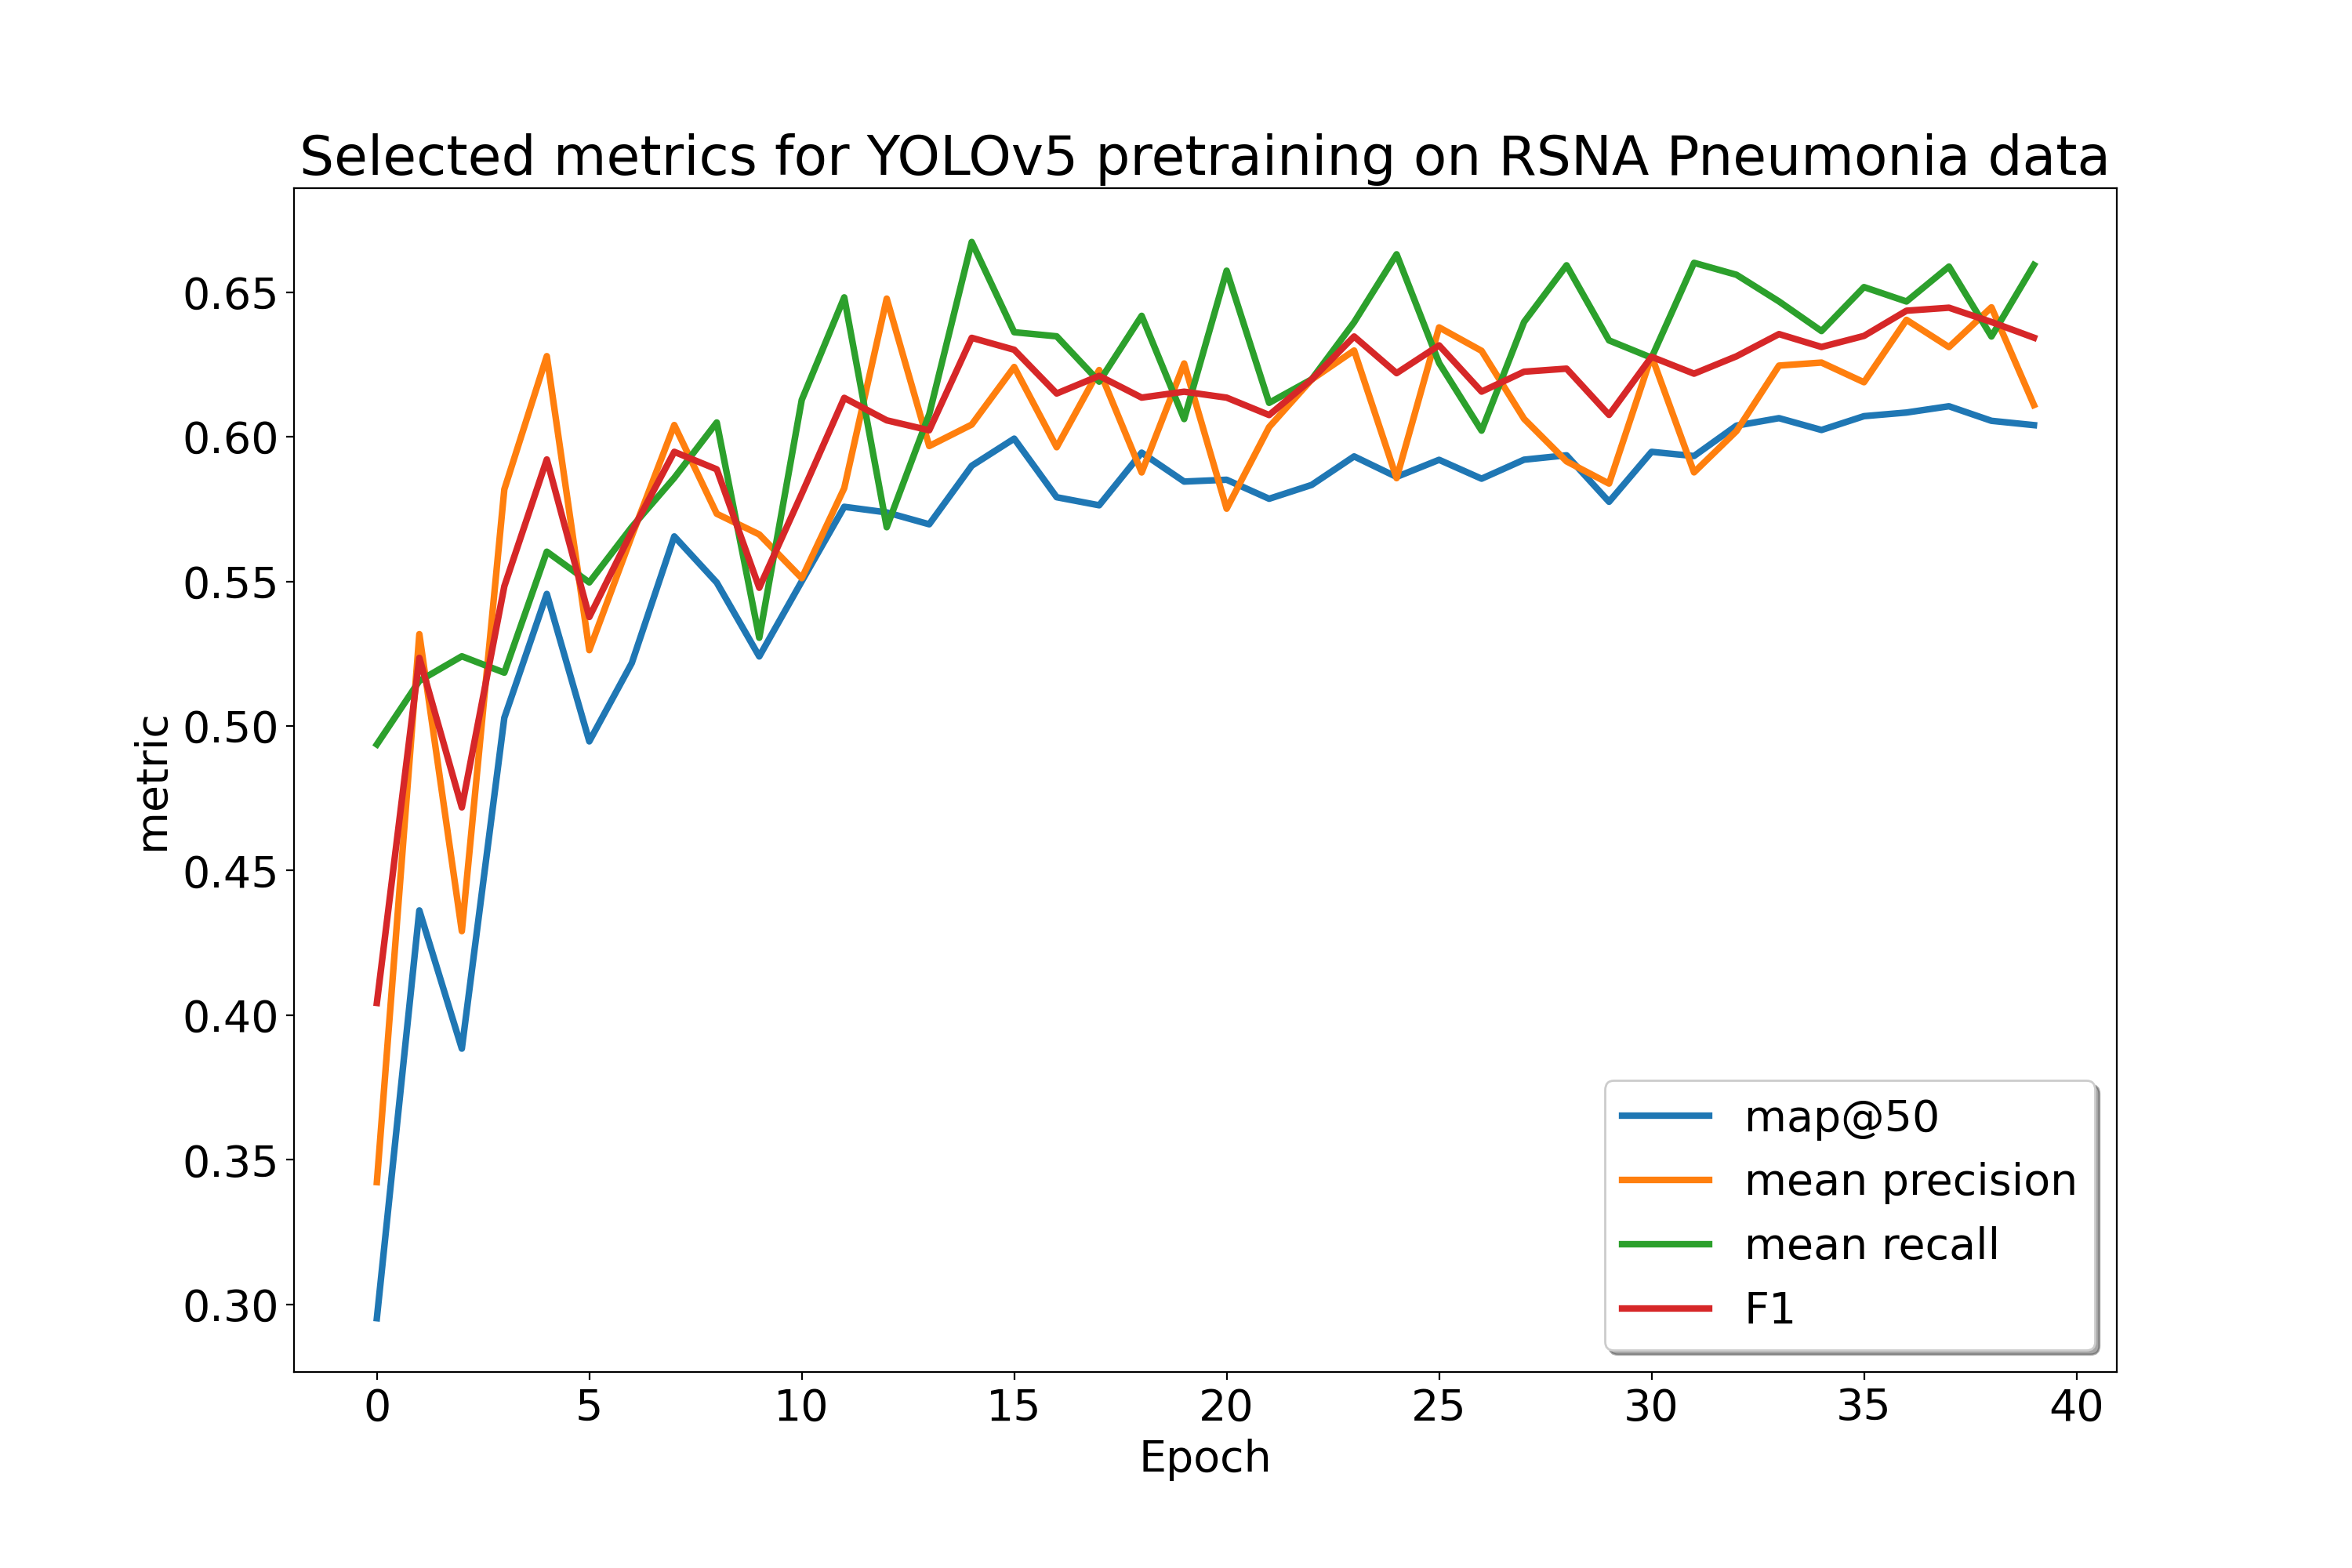
\includegraphics[width=\linewidth]{img/metrics_giou_pretrained_yolo_40.png}
		\caption{Validation results for the \ac{YOLO} pretraining.}
		\label{fig:yolo_pretraining_results}
	\end{minipage}
	\begin{minipage}[b]{.5\linewidth} % [b] => Ausrichtung an \caption
		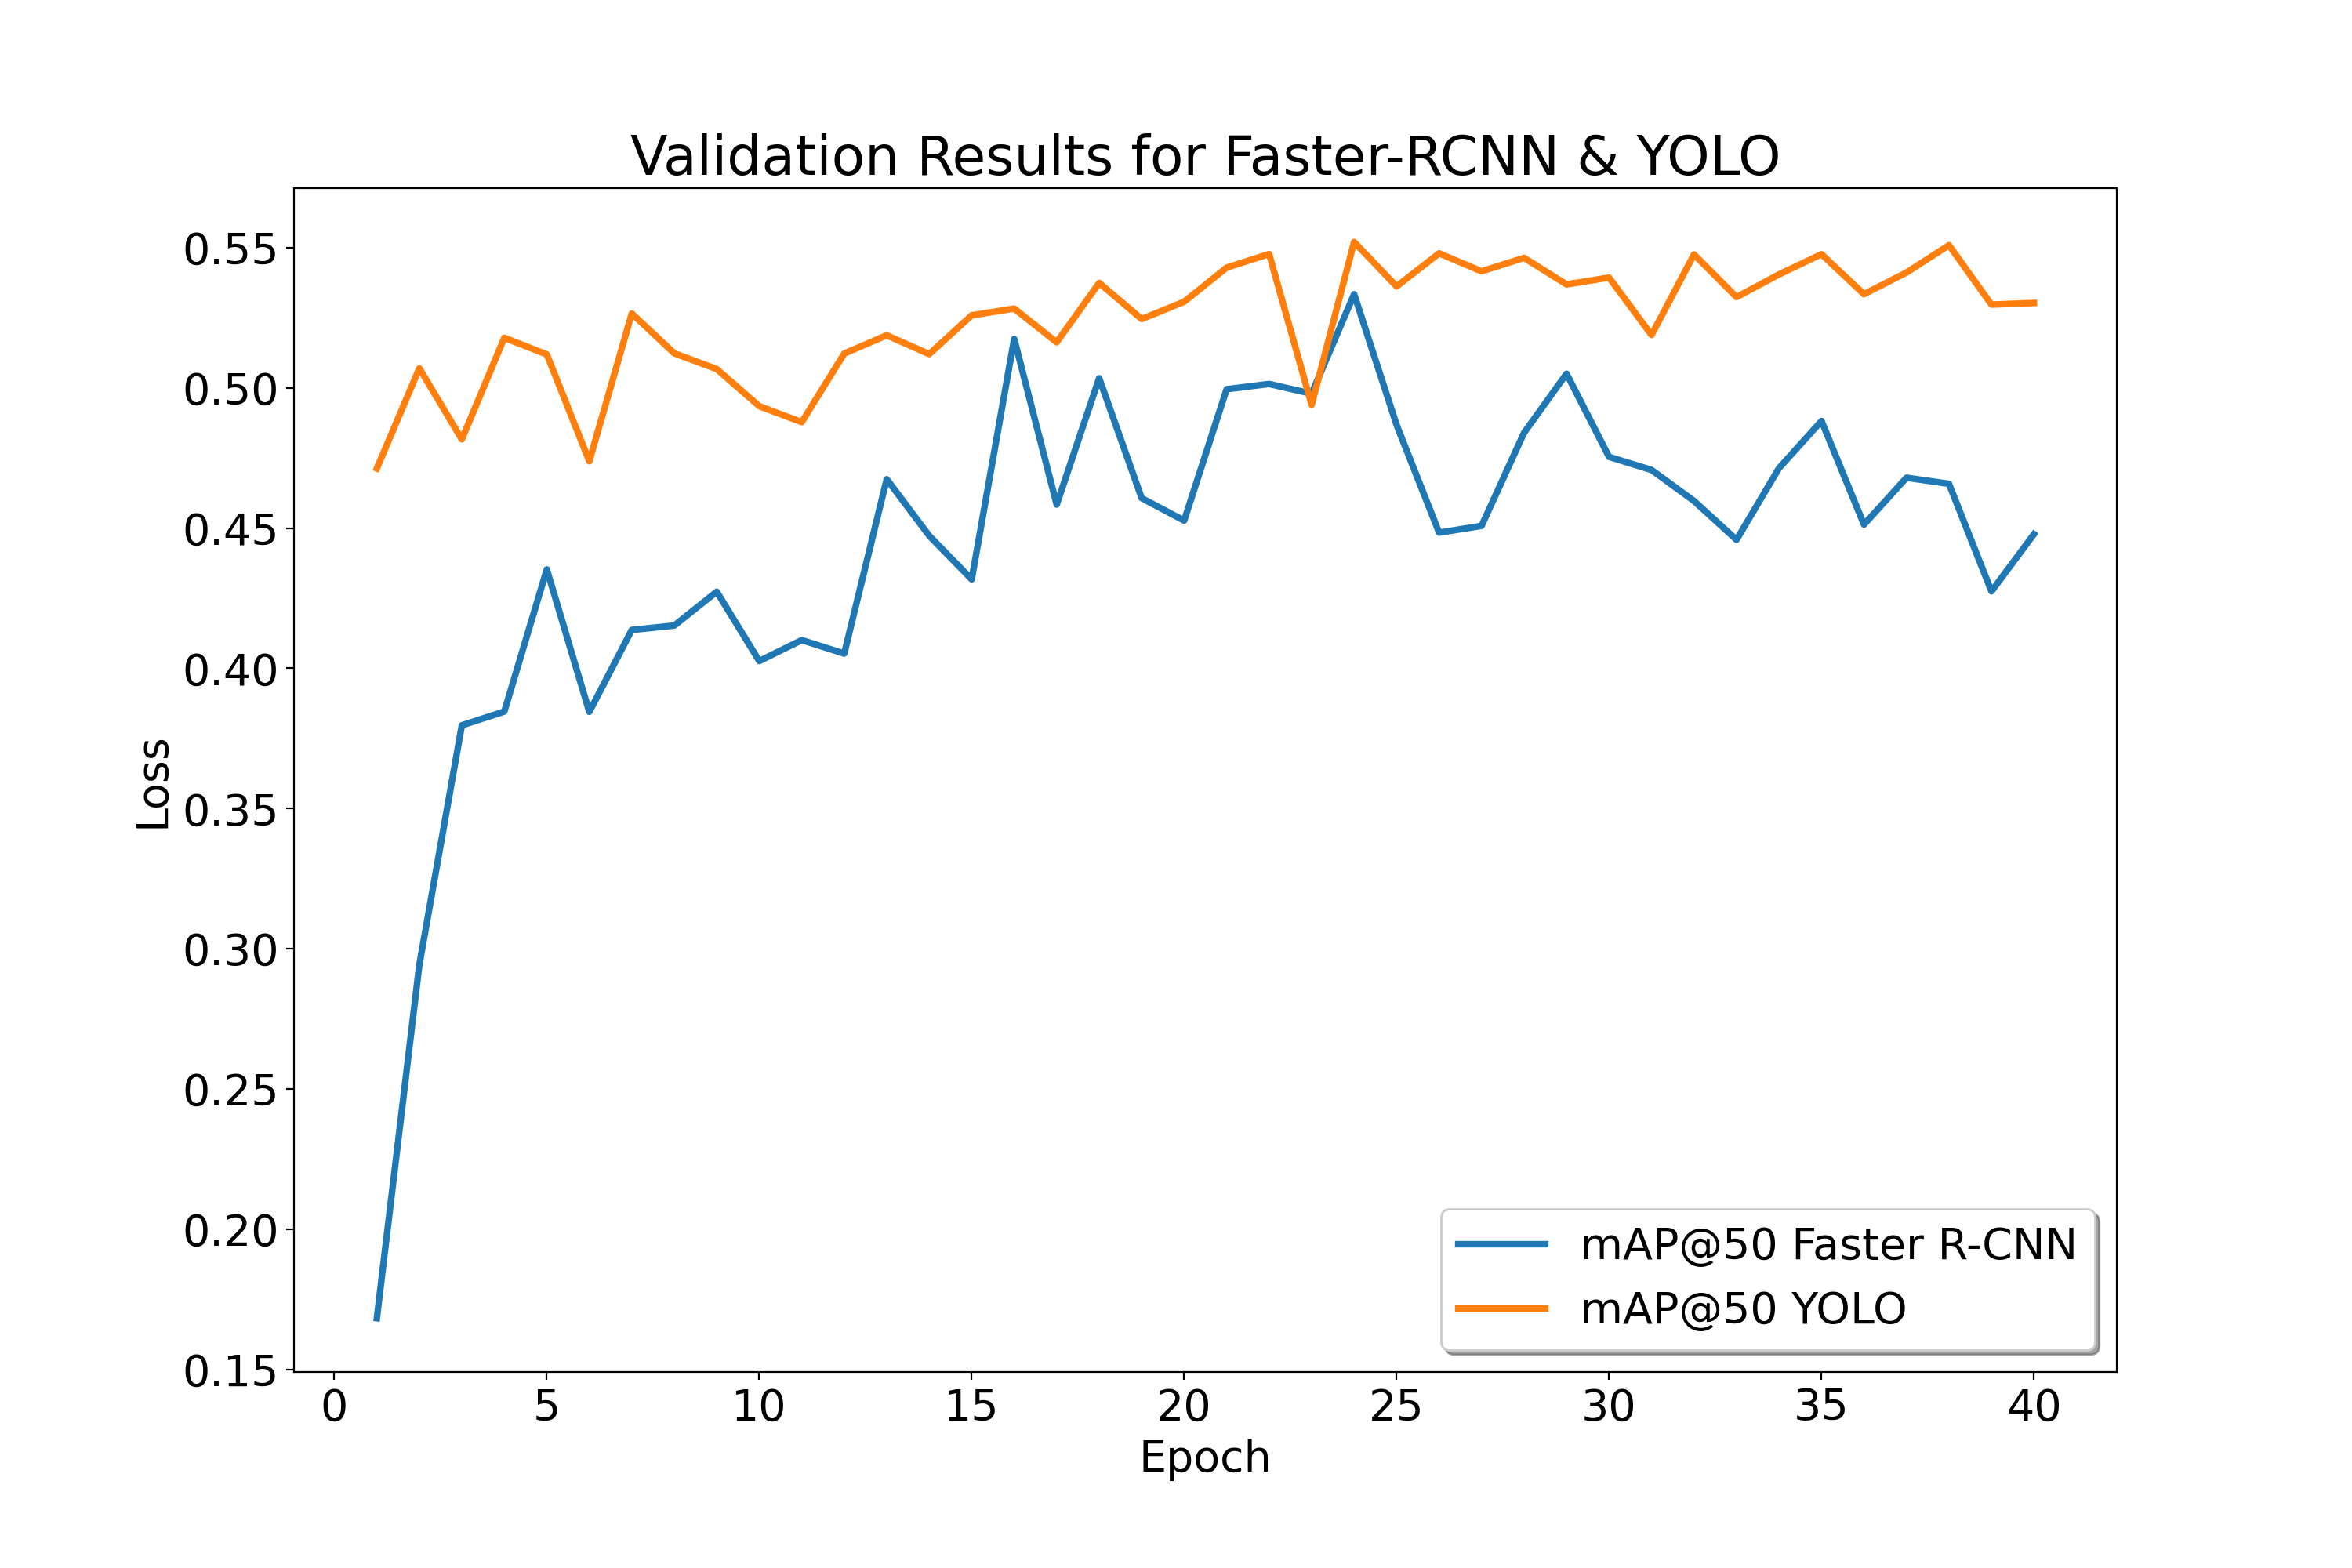
\includegraphics[width=\linewidth]{img/eval_results_ap_only_fasterrcnn_yolo.png}
		\caption{Validation results on the SIIM COVID-19 data.}
		\label{fig:yolo_frcnn_results}
	\end{minipage}
\end{figure*}
The final validation results during training for both detection models on the COVID-19 dataset can be found in \ref{fig:yolo_frcnn_results}. The figure shows that we see only a slow increase in \ac{mAP}@$.50$ for the \ac{YOLO} model which is mainly caused by the pretraining. In contrast, the Faster \ac{R-CNN} model shows a similar pattern like the \ac{YOLO} in pretraining where with increasing number of epochs the metric values flatten out after a heavy increase in the first epochs. In general, we could observe that the \ac{YOLO} model shows better results with a \ac{mAP}@$.50$ of $\approx 55\%$, whereas the Faster \ac{R-CNN} reaches $\approx 53\%$ in its best epoch. As already indicated in the training sections, we could observe a slight overfit of the model leading to a decreasing score again. This phenomenon might be caused by the limited data available or a too long training. Due to limited time capacity we did not analyzed this behavior in more detail and leave this open for further research, including hyper-parameter tuning and cross-validation methods.
However, we choose the best observed models for our final implementation of the COVID-19 detection. In more detail we used the \ac{YOLO} model checkpoint at epoch 26 and the Faster \ac{R-CNN} model checkpoint at epoch 23.

Finally, table \ref{table:final_results} shows extended evaluation results of the models including also the ensemble performance on a held-out consisting of 859 examples. 
\begin{table}[h]
	\begin{tabular}{l|l|l|l}
		&    Faster R-CNN          &         YOLO             &  Ensemble \\ \hline
		mAP@.50			& \multicolumn{1}{l|}{0.409} & \multicolumn{1}{l|}{0.345} & \textbf{0.451}  \\
		F1-score		& \multicolumn{1}{l|}{0.547} & \multicolumn{1}{l|}{0.477} & \textbf{0.560} \\
		mean Recall		& \multicolumn{1}{l|}{0.503} & \multicolumn{1}{l|}{0.450} & \textbf{0.530} \\
		mean Precision	& \multicolumn{1}{l|}{\textbf{0.603}} & \multicolumn{1}{l|}{0.506} & 0.594 \\
	\end{tabular}
	\centering
	\caption{Final evaluation results on the held-out test set.}
	\label{table:final_results}
\end{table}

In addition to the \ac{mAP}@$.50$ we took F1, mean Recall and mean Precision into consideration. The results show clearly, that surprisingly, the \ac{YOLO} model performs worse than the Faster \ac{R-CNN}, which the validation results during training would not have let expected. However, this reflects pretty much the model performances obtained in other research, where the Faster \ac{R-CNN} performs in average always better than \ac{YOLO}, where the advantages in \ac{YOLO} lays in the inference speed through its one-shot capability. Fortunately, we could see that combining both models through our ensemble approach leads to the best performance in all selected metrics except the mean Precision, where the Faster \ac{R-CNN} performs slightly better.

\begin{figure*}[h!]
	\centering
	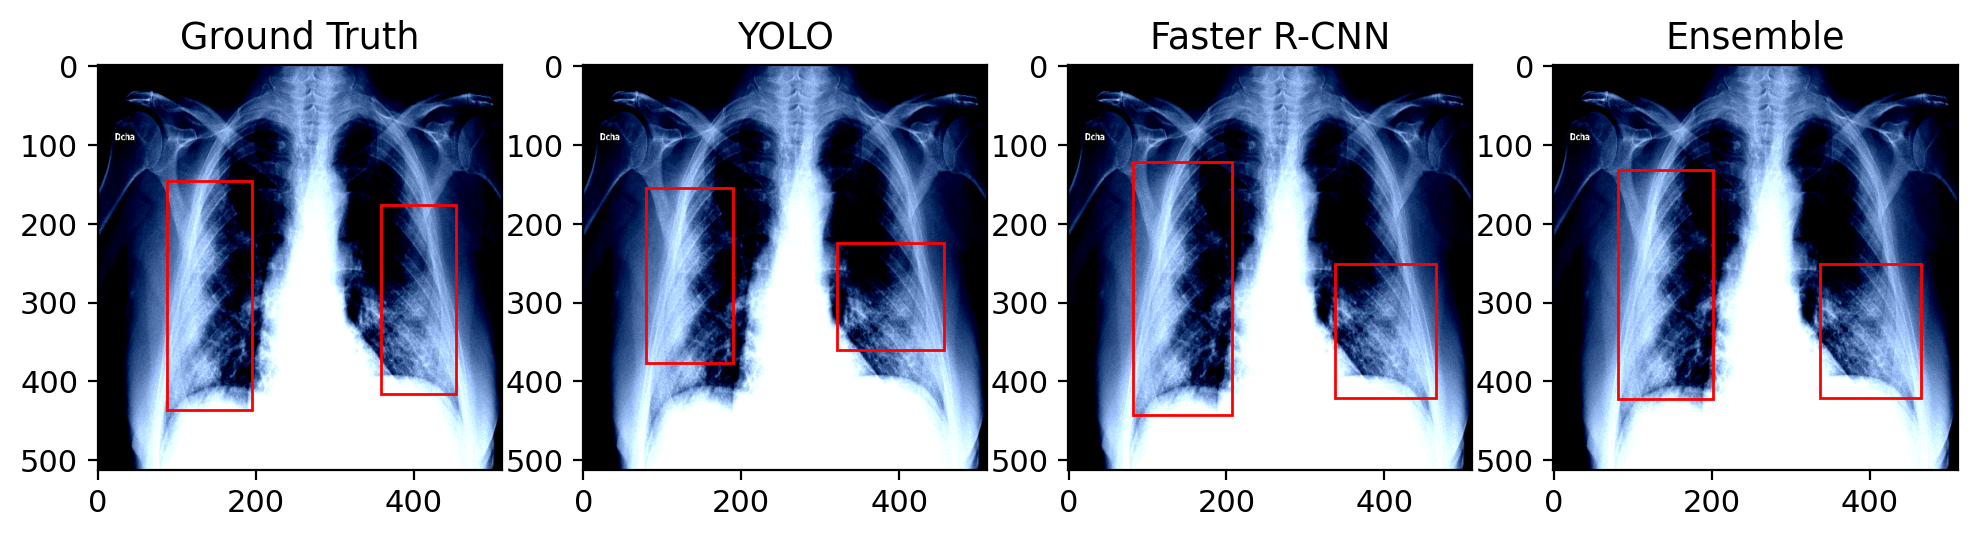
\includegraphics[width=0.6\linewidth]{img/combo.png}
	\caption{Prediction Results on a random examples from the held-out set.}
	\label{fig:combo_eval}
\end{figure*}
To show also a qualitative comparison, figure \ref{fig:combo_eval} shows five different samples from the held-out set and their corresponding predictions of the Faster \ac{R-CNN}, \ac{YOLO} and Ensemble model. It can be observed that both the models already detect affected regions very well, especially in terms of absolute position and agree in most of the predictions, but also struggle in finding the perfect magnitudes of the boxes. Further, the results reveal also some problems of the models as visualized in the third and fifth example, where both models and ultimately the ensemble fails on detecting rather small bounding boxes. In addition, the \ac{YOLO} predicts in most of the cases smaller boxes relative to the Faster \ac{R-CNN} leading to final results that are mainly driven by the latter predictions despite we designed the weights such that both model should contribute equally which is shown in the fifth example of figure \ref{fig:combo_eval}. 

To conclude this section, we showed that both models perform well on the task of detecting COVID-19 affected regions on chest X-rays, reaching the best results by combining a \ac{YOLO} and Faster \ac{R-CNN} model by a confident score dependent bounding box fusion, but still letting some open room for improvements (as will be discussed in chapter \ref{chapter:conclusion}).

\section{Evaluation of Study-Level Model}
\sectionauthor{Written by Torben Krieger}